\subsection{使用器具}
	ツェナーダイオードの特性実験の使用機材を以下の\wtab{zenerDiode_apparatus}に示す。
	\begin{table}[hbt]
		\centering
		\caption{使用器具}
		\begin{tabular}{|c||c|c|c|} \hline
				使用器具名 & 製造元 & 型番 & 製造番号(管理番号)\\ \hline
				電流計(ミリアンペア計)1 & YOKOGAWA & E-CLASS 1.0 & 48-2 \\ \hline
				電流計(ミリアンペア計)2 & YOKOGAWA & E-CLASS 1.0 & 578 \\ \hline
				電圧計 & YOKOGAWA & E-CLASS 1.0 & 278-20 \\ \hline
				電源装置 & YOKOGAWA & PA1811 & L69-000668 \\ \hline
				可変抵抗3 & TOKUSHU DENKI KOGYOSHO & S-3 & 3201 \\ \hline
		\end{tabular}
		\label{tab:zenerDiode_apparatus}
	\end{table}

%	% %	%	%	% %	% %	%	%	% %	% %	%	%	% %	% %	%	%	% %	% %	%	%	% %	% %	%	%	% %	% %	%	%	%
\subsection{ツェナーダイオードの特性}
\subsubsection{実験方法}
	ツェナーダイオードの特性計測に用いた回路を\wfig{zenerDiode1_circuit} に示す。

	\begin{figure}[!h]
    \centering
    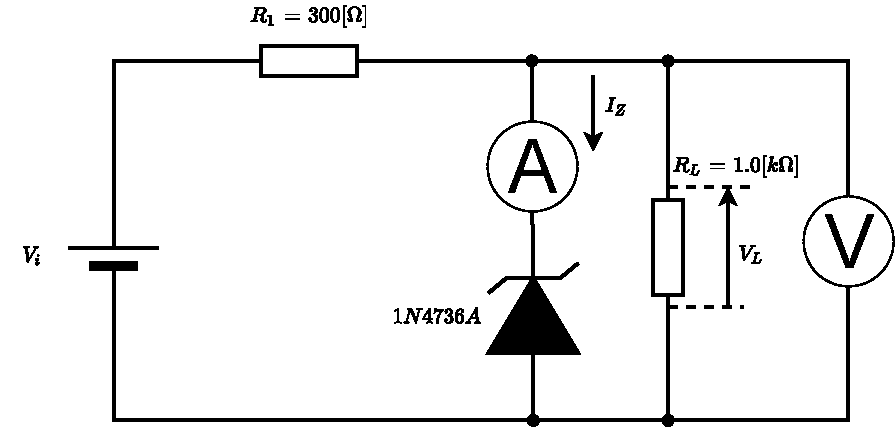
\includegraphics[width=10cm]{./pdfs/zener_diode1.pdf}
    \caption{ツェナーダイオード特性の回路図}
    \label{fig:zenerDiode1_circuit}
  \end{figure}
	
  この実験では直流電源の電圧$V_i$を18~0 V まで1 V ずつ減少させた。
  そのときの電流$I_Z$,電圧$V_L$を計測した。

\subsubsection{結果}
	計測して得られたデータを\wtab{zenerDiode1_result} に示す。
	また\wtab{zenerDiode1_result} から作成したグラフを\wfig{zener_Vi-VLIZ} に示す。
	この表から,入力電圧$V_i$が0~8 V ではツェナーダイオードに電流が流れていないことが分かる。
	電圧$V_L$は,ツェナーダイオードと並列に接続されている抵抗の電圧であり,ツェナーダイオードの電圧$V_D$でもある。
	電圧$V_L$が6.61 V のとき,ツェナーダイオードは電流を流し始めている。
	その後,入力電圧$V_i$が増加しても,$V_L$はあまり変化していないことが分かる。
	また,$V_L$の変化が減ると同時に,ツェナーダイオードに流れる電流$I_Z$が増加していることが分かる。

	\begin{table}[hbt]
		\centering
		\caption{ツェナーダイオードの特性の計測結果}
		\begin{tabular}{|c|c|c|}
		\hline
		電圧$V_i$ [V] & 電圧$V_L$ [V] & 電流$I_Z$ [mA] 			 \\ \hline
		0            & 0            & 0             \\ \hline
		1            & 0.78         & 0             \\ \hline
		2            & 1.54         & 0             \\ \hline
		3            & 2.28         & 0             \\ \hline
		4            & 3.06         & 0             \\ \hline
		5            & 3.82         & 0             \\ \hline
		6            & 4.58         & 0             \\ \hline
		7            & 5.35         & 0             \\ \hline
		8            & 6.1          & 0             \\ \hline
		9            & 6.61         & 1             \\ \hline
		10           & 6.64         & 4.2           \\ \hline
		11           & 6.66         & 7.8           \\ \hline
		12           & 6.69         & 10.8          \\ \hline
		13           & 6.72         & 16.2          \\ \hline
		14           & 6.74         & 17.6          \\ \hline
		15           & 6.76         & 20.8          \\ \hline
		16           & 6.78         & 24.2          \\ \hline
		17           & 6.8          & 27.8          \\ \hline
		18           & 6.82         & 30.8          \\ \hline
		\end{tabular}
		\label{tab:zenerDiode1_result}
	\end{table}

	\begin{figure}[!h]
    \centering
    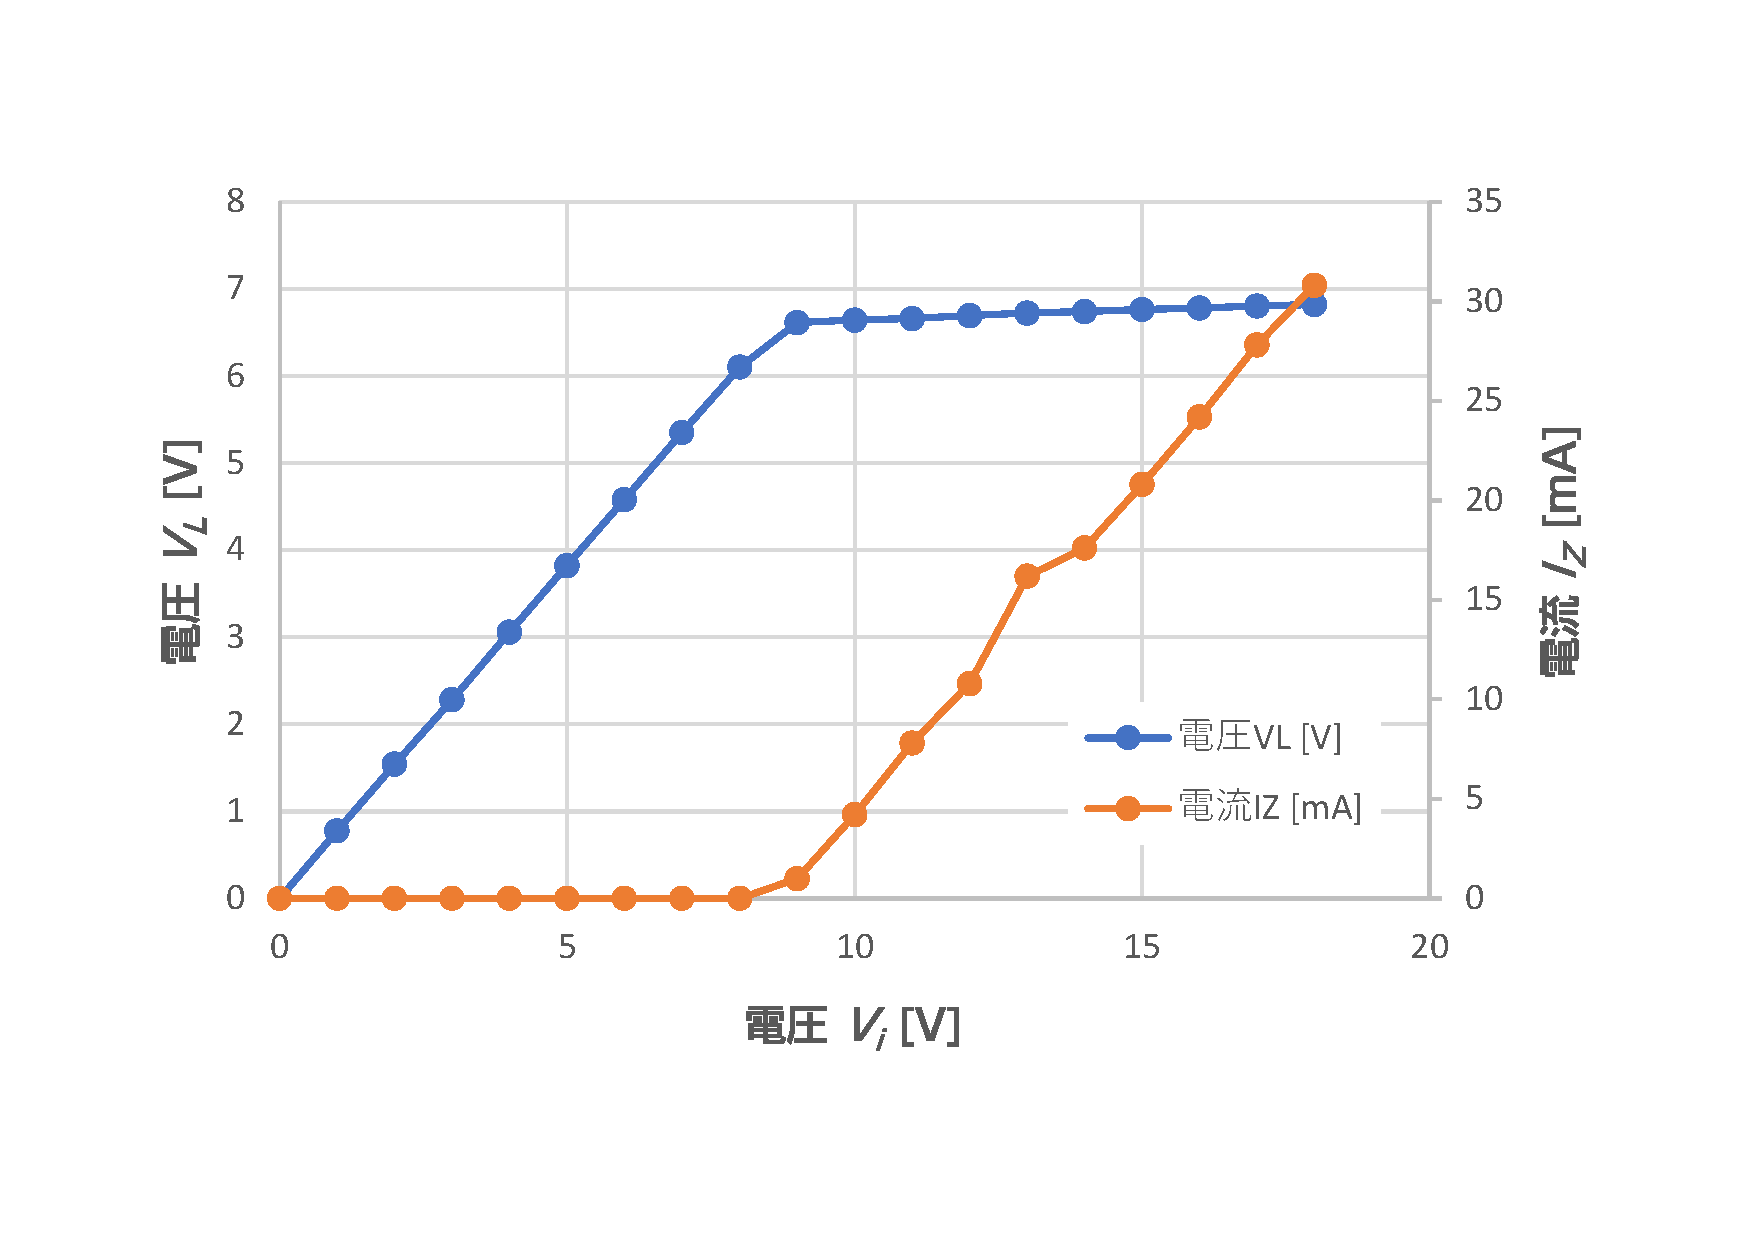
\includegraphics[width=13cm]{./figs/G-zener_Vi-VLIZ.pdf}
    \caption{入力電圧とツェナーダイオードの電圧電流特性}
    \label{fig:zener_Vi-VLIZ}
  \end{figure}

\subsubsection{考察}
	\begin{enumerate}
		\item ツェナーダイオード 1N4736A のデータシートでツェナー電圧を調べ,実験結果と比較して考察せ
		よ。\\

		1N4736A のデータシート\cite{web:1N4736A} によると, ツェナーダイオード 1N4736A のツェナー電圧は Typ. 6.8 V (25℃)である。
		\wtab{zenerDiode1_result} より,$V_L$が6.61~6.82 V の間でツェナーダイオードに電流が流れていることが分かる。
		電流が流れている間の$V_L$の平均値は 6.72 V である。
		データシートの値と計測値にほとんど差がなく,計測が成功していると考えられる。

		\item ツェナーダイオードはどのような場合に用いられるか説明せよ。\\
  
		ツェナーダイオードは一定電圧を保つダイオードである。
		マイクロマウスなどのロボットは,壁やラインを検知するために,フォトリフレクタを用いる。
		フォトリフレクタは,LEDとフォトダイオード(フォトトランジスタ)で構成される。
		LEDを発光させ,反射光をフォトダイオードで強度から,距離や色を検知するものである。
		このとき,LEDの出力が一定でないと正確なデータを計測できず,ロボットがパフォーマンスを発揮しきれないことがある。
		そこで,ツェナーダイオード用いることで,各LEDにかかる電圧を一定にでき,LEDの出力を安定化させることができる。

  	\item VL − VZ 特性のグラフを書き,ツェナー電圧 VZ を説明せよ。\\
   
		\wfig{zener_VL-IZ} はツェナーダイオードの電圧電流特性とツェナー電圧を示したグラフである。
		ツェナー電圧は $V_L = $6.8 V と設定した。
		ツェナー電圧とツェナーダイオードの電圧電流特性のグラフはほとんど一致している。
		このことから,このツェナーダイオードのツェナー電圧は約6.8 V だと考えられる。
   
		\begin{figure}[!h]
			\centering
			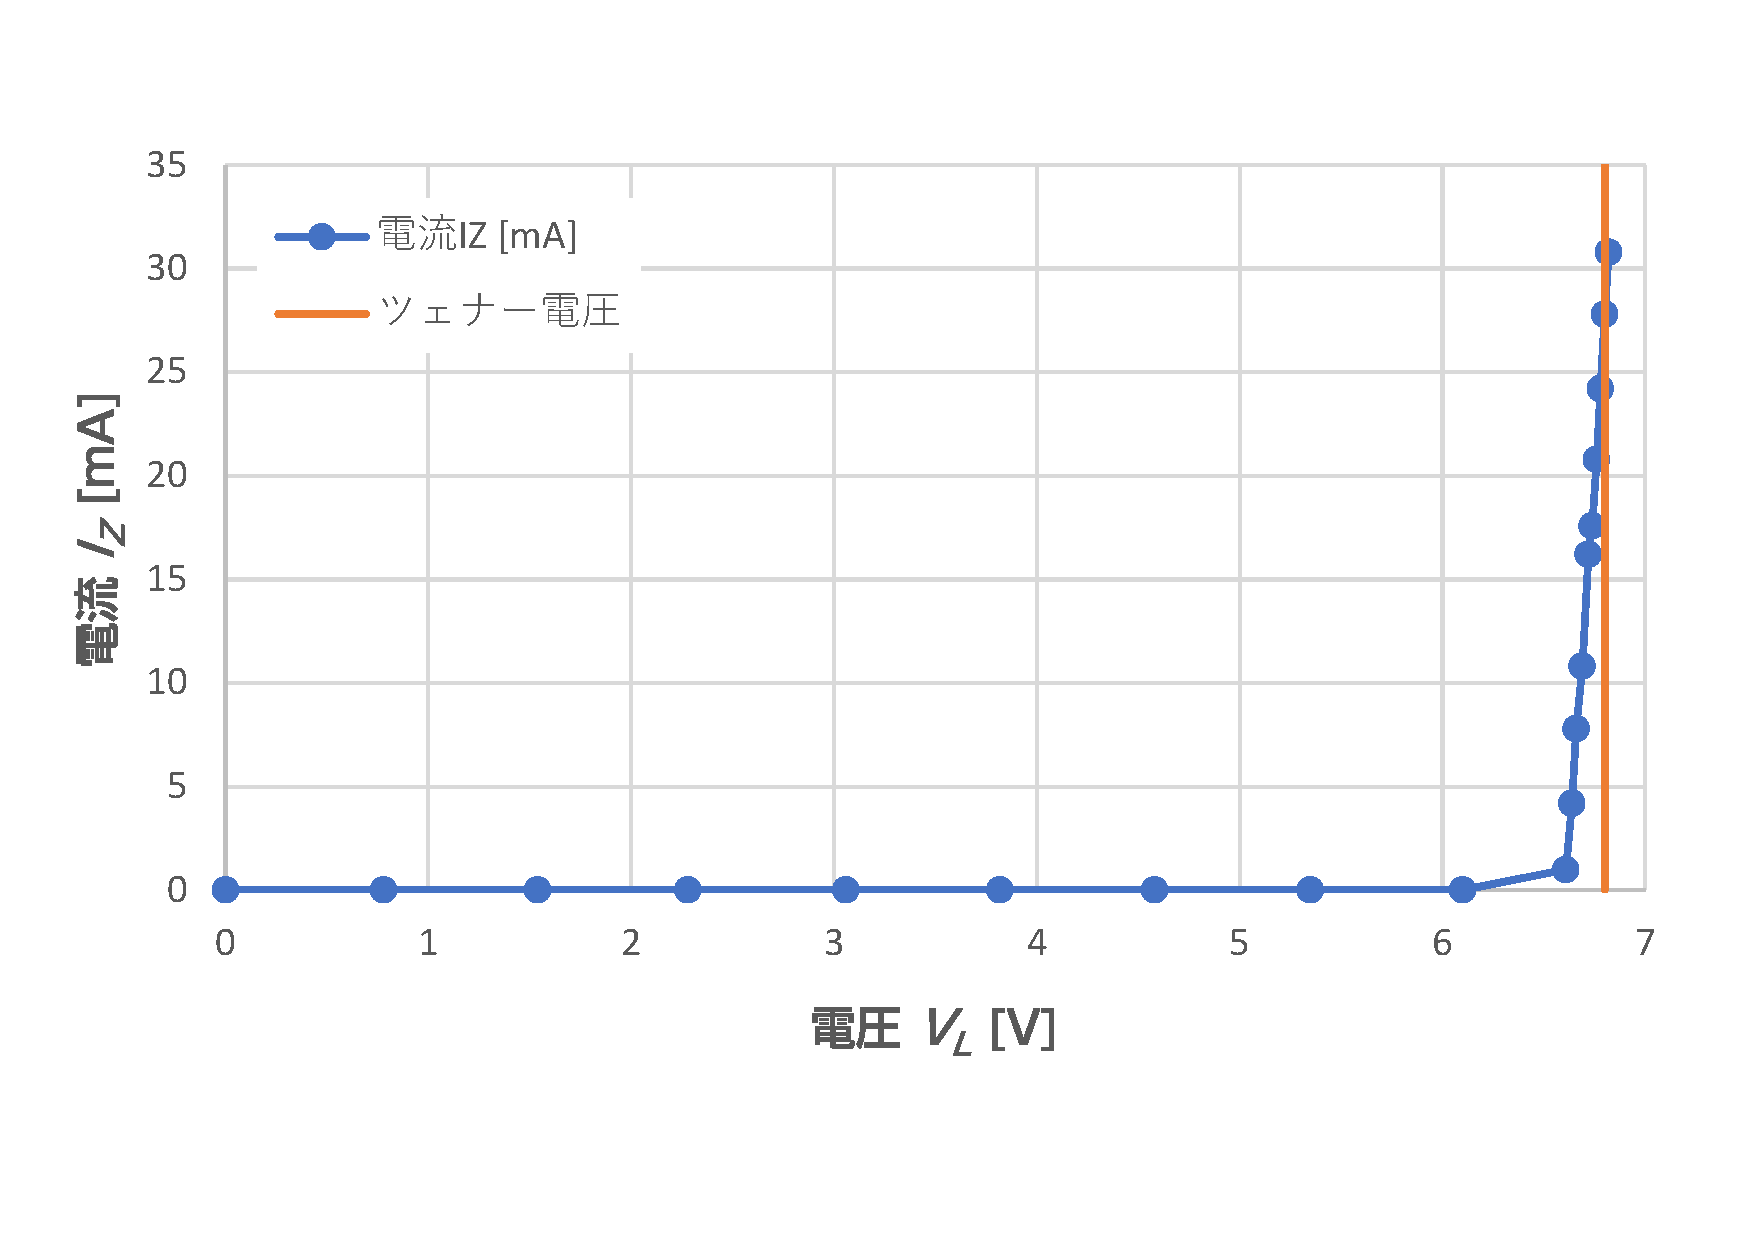
\includegraphics[width=13cm]{./figs/G-zener_VL-IZ.pdf}
			\caption{ツェナーダイオードの電圧電流特性とツェナー電圧}
			\label{fig:zener_VL-IZ}
		\end{figure}

   	\item 各グラフから入出力特性を考察せよ。\\
     
		\wfig{zener_VL-IZ} より,ツェナーダイオードは一定電圧を超えると,急激に電流を通すようになる特性が考えられる。
		また,急激に電流を通すようになることから,急激に抵抗値が低下しているとも考えられる。
		\wfig{zener_Vi-VLIZ} より,ツェナーダイオードは一定電圧を保つ特性があると考えられる。
		
	\end{enumerate}

%	% %	%	%	% %	% %	%	%	% %	% %	%	%	% %	% %	%	%	% %	% %	%	%	% %	% %	%	%	% %	% %	%	%	%
\subsection{ツェナーダイオード定電圧回路}
\subsubsection{実験方法}
	ツェナーダイオード定電圧特性の計測に用いた回路を\wfig{zenerDiode2_circuit} に示す。

	\begin{figure}[!h]
		\centering
		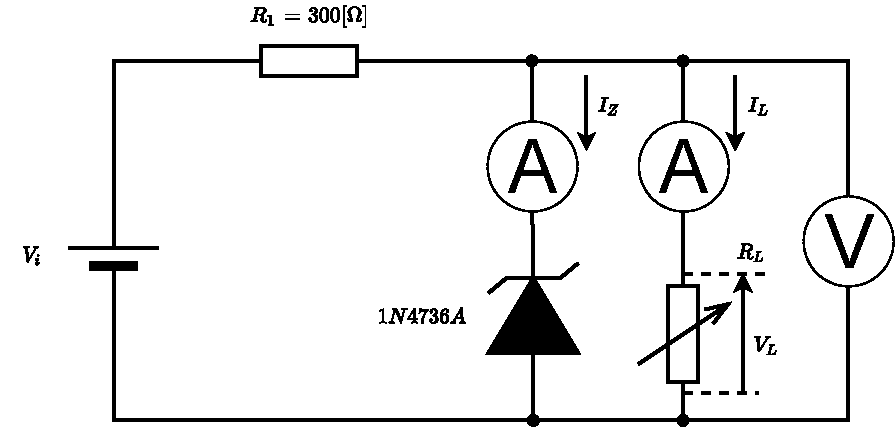
\includegraphics[width=10cm]{./pdfs/zener_diode2.pdf}
		\caption{ツェナーダイオード定電圧特性の回路図}
		\label{fig:zenerDiode2_circuit}
	\end{figure}

	この実験では直流電源の電圧$V_i$を15 V に固定し,可変抵抗$R_L$を変化させて,ツェナー電流$I_Z$が2~22 mA まで2 mA ずつ増加するようにした。
	そのときの出力電圧$V_L$,出力電流$I_L$を計測した。

\subsubsection{結果}
	計測して得られたデータを\wtab{zenerDiode2_result} に示す。
	また\wtab{zenerDiode2_result} から作成したグラフを\wfig{zener_IZ-VL} と\wfig{zener_IZ-IL} に示す。
	\wfig{zener_IZ-VL} から,ツェナー電流$I_Z$に関わらず,ツェナー電圧$V_Z$はほとんど一定であることが分かる。
	\wfig{zener_IZ-IL} から,ツェナー電流$I_Z$が増加すると,$I_L$が減少していることが分かる。
	また,$I_L$は$I_Z$に比例して減少していることも分かる。

	\begin{table}[hbt]
		\centering
		\caption{ツェナーダイオードの定電圧特性の計測結果}
		\begin{tabular}{|c|c|c|}
		\hline
		電流$I_Z$ [mA] & 電流$I_L$ [mA] & 電圧$V_L$ [V] \\ \hline
		2                        & 25.85           & 6.6            \\ \hline
		4                        & 23.9            & 6.62           \\ \hline
		6                        & 21.9            & 6.62           \\ \hline
		8                        & 19.75           & 6.64           \\ \hline
		10                       & 17.55           & 6.68           \\ \hline
		12                       & 15.6            & 6.7            \\ \hline
		14                       & 13.6            & 6.76           \\ \hline
		16                       & 11.65           & 6.76           \\ \hline
		18                       & 9.7             & 6.76           \\ \hline
		20                       & 7.75            & 6.78           \\ \hline
		22                       & 5.6             & 6.78           \\ \hline
		\end{tabular}
		\label{tab:zenerDiode2_result}
	\end{table}

	\begin{figure}[!h]
		\centering
		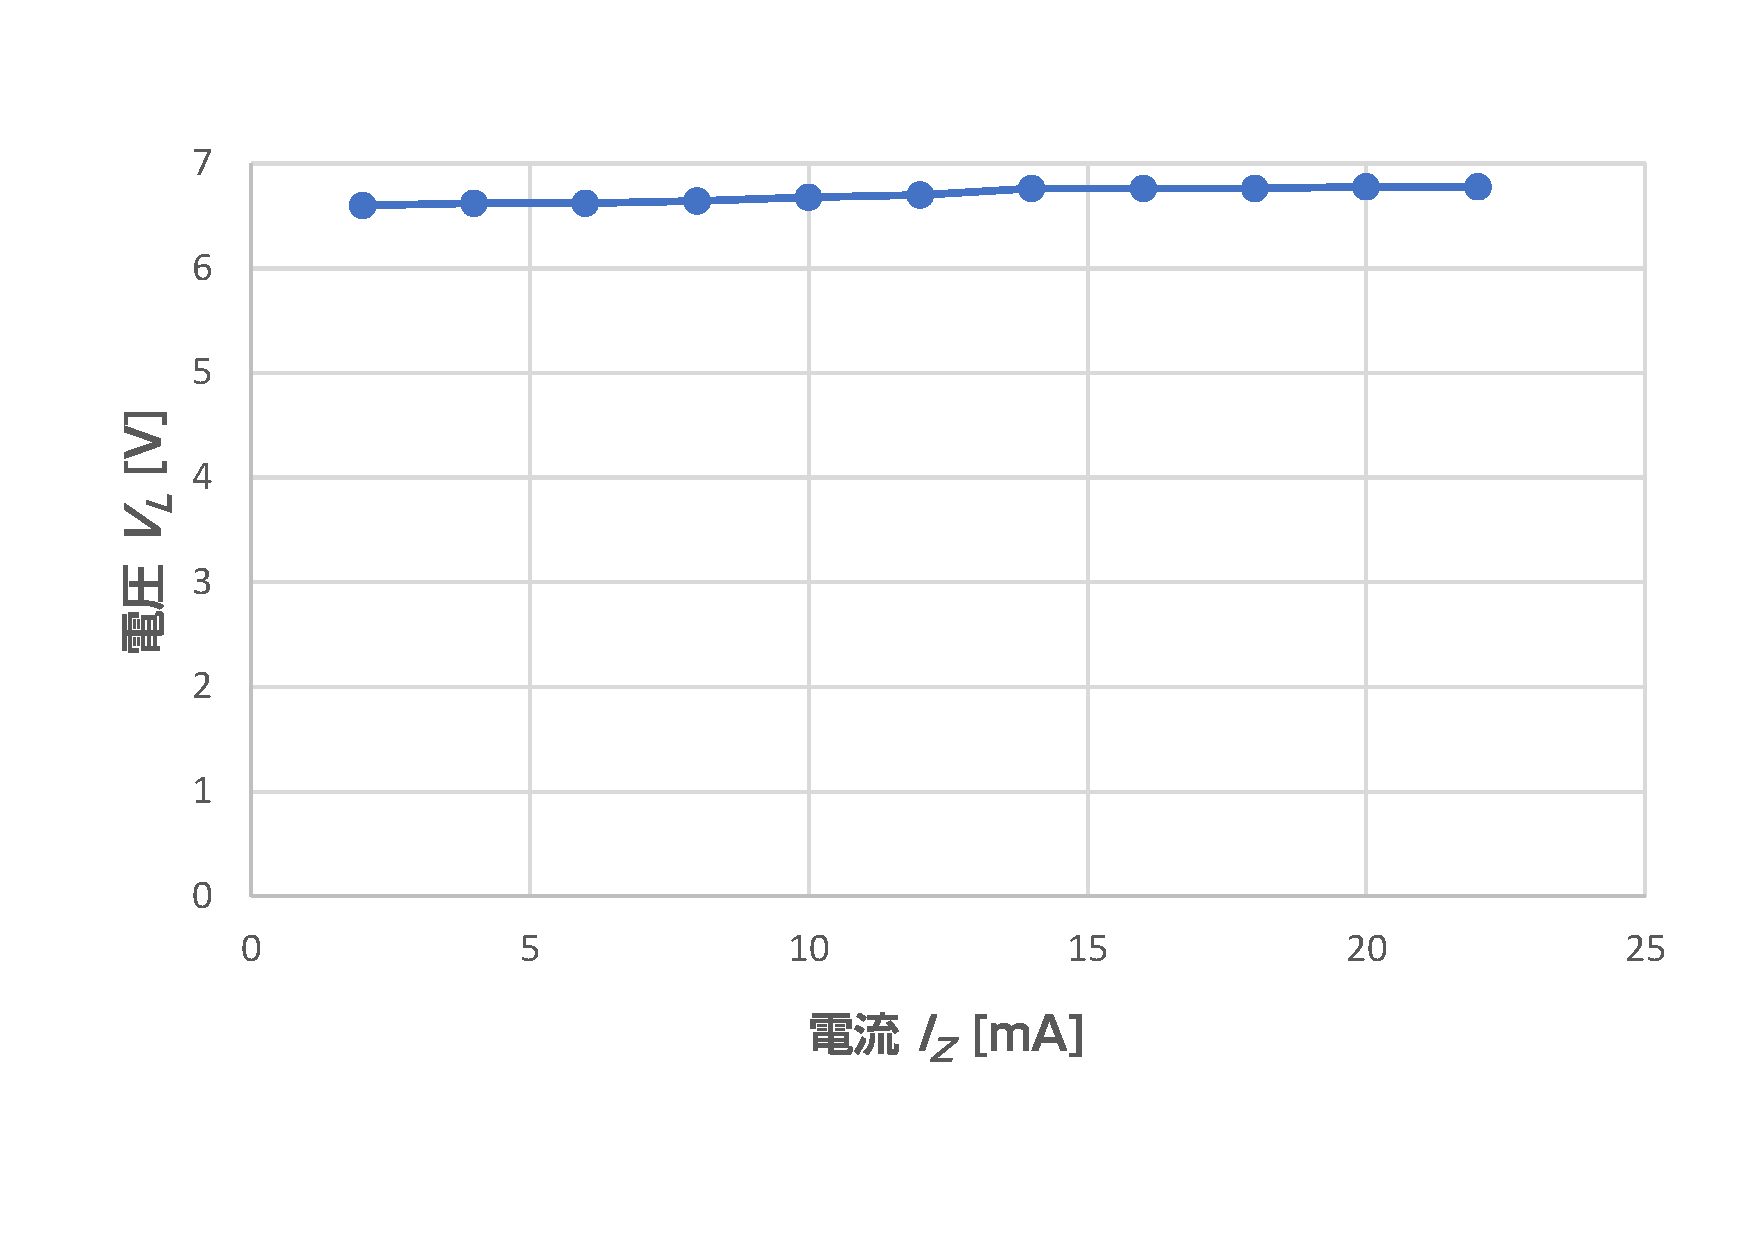
\includegraphics[width=13cm]{./figs/G-zener_IZ-VL.pdf}
		\caption{ツェナーダイオードの電流出力電圧特性}
		\label{fig:zener_IZ-VL}
	\end{figure}
	\begin{figure}[!h]
		\centering
		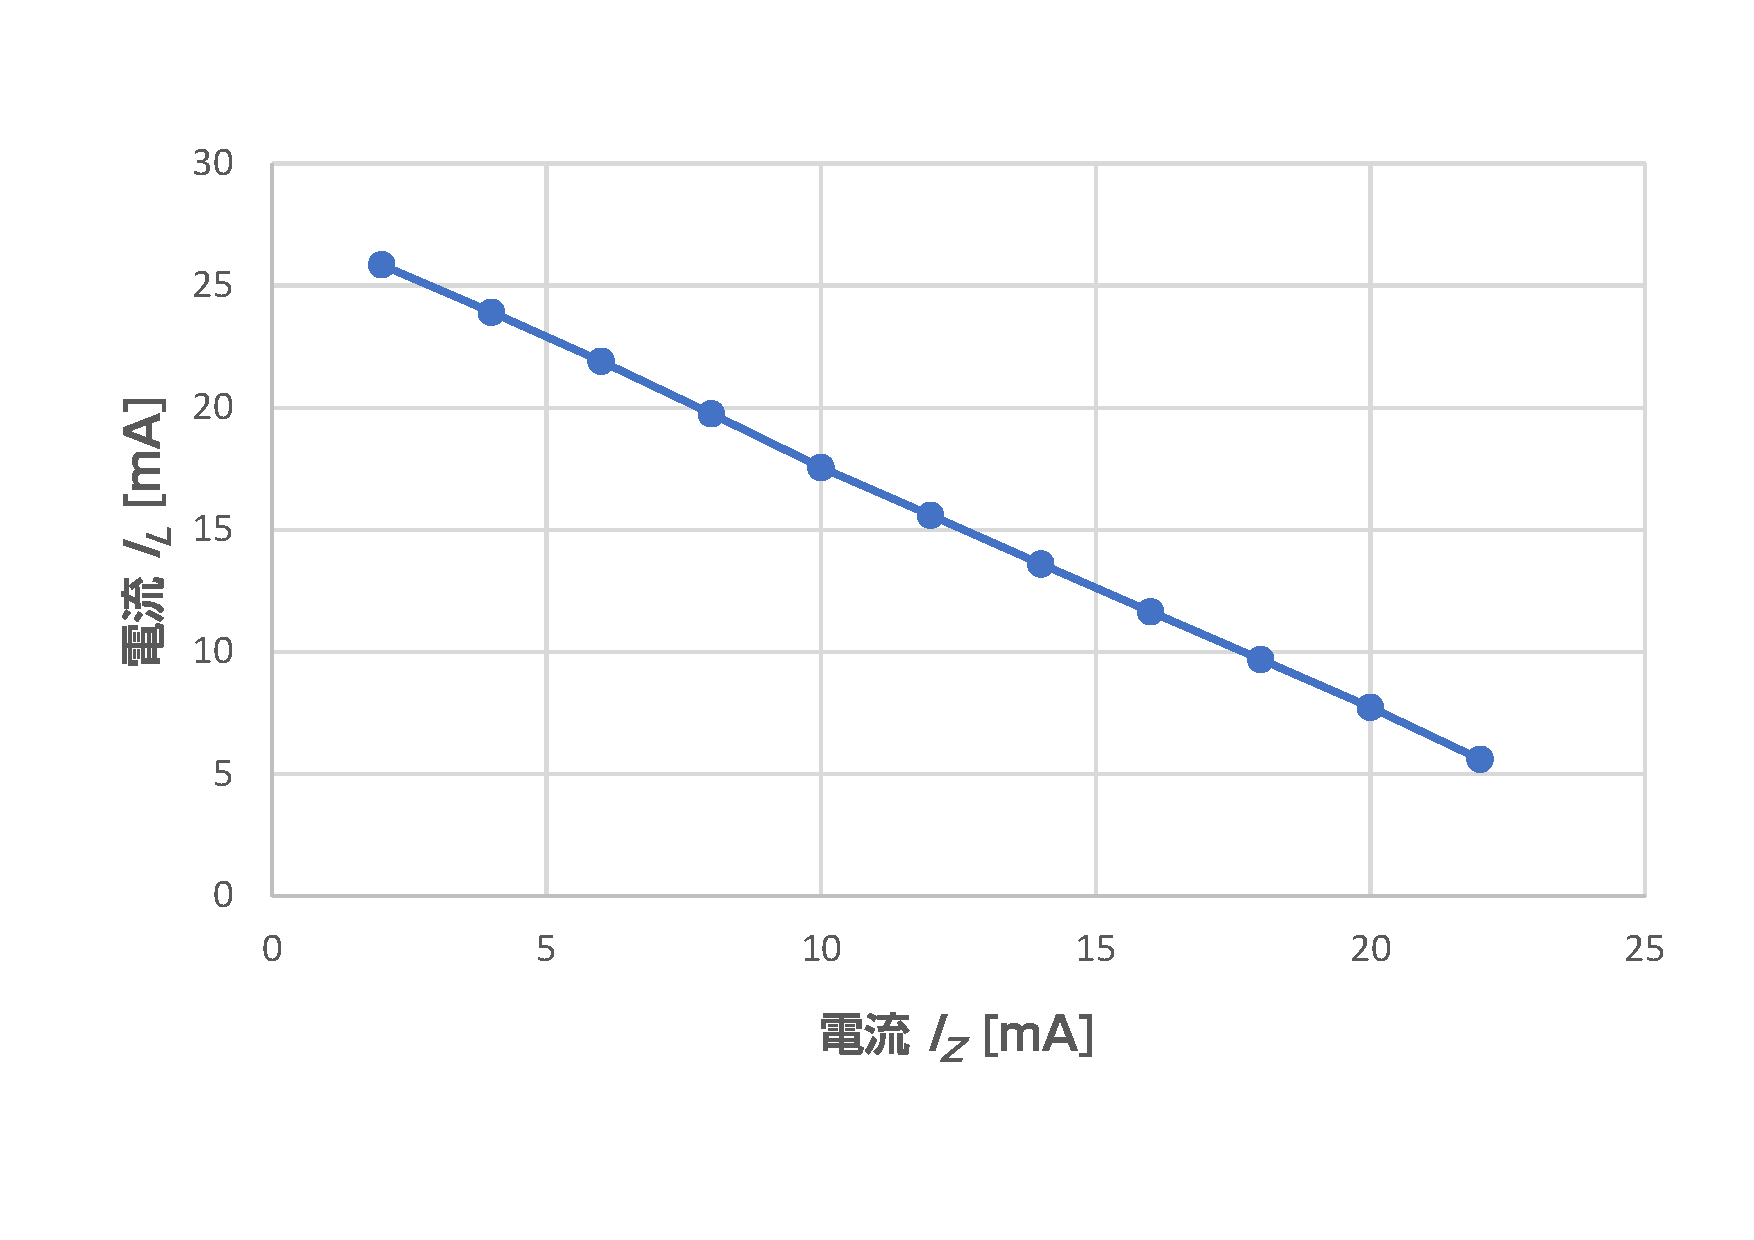
\includegraphics[width=13cm]{./figs/G-zener_IZ-IL.pdf}
		\caption{ツェナーダイオードの電流出力電流特性}
		\label{fig:zener_IZ-IL}
	\end{figure}

\subsubsection{考察}
	\begin{enumerate}
		\item 測定結果から,$R_L$,$R_Z$,およびこれらの合成抵抗 $R_A$ を算出せよ。\\
  
		\wfig{risou2} はツェナーダイオード定電圧回路の等価回路である。
		$ZD$は理想ツェナーダイオードであり,$R_Z$はツェナーダイオードの抵抗成分を示す。
		
				\begin{figure}[!h]
					\centering
					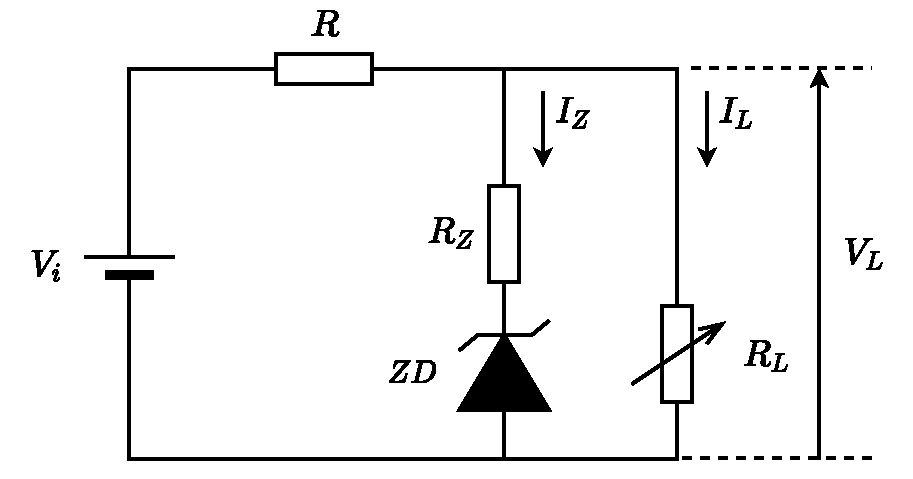
\includegraphics[width=8.2cm]{./pdfs/risou2.pdf}
					\caption{ツェナーダイオード定電圧回路の等価回路}
					\label{fig:risou2}
				\end{figure}
		
		$R_Z$,$R_L$は以下の式で求められる。
		\begin{align}
			R_Z &= \frac{V_L}{I_Z} \nonumber \\
			R_L &= \frac{V_L}{I_L} \nonumber
		\end{align}
		合成抵抗$R_A$は以下の式で求められる。
		\begin{equation}
			R_A = \frac{R_Z R_L}{R_Z + R_L} \nonumber
		\end{equation}
		これらの計算をそれぞれの計測点で行った結果を\wtab{resistance_calc1} に示す。
		\wtab{resistance_calc1} から合成抵抗$R_A$の抵抗値は,ほとんど変化していないと考えられる。

		\begin{table}[hbt]
			\centering
			\caption{$R_Z$,$R_L$,$R_A$の計算結果}
			\begin{tabular}{|c|c|c|c|}
			\hline
			電流$I_Z$ [mA] & 抵抗値$R_Z$ [k$\Omega$] & 抵抗値$R_L$ [k$\Omega$] & 合成抵抗$R_A$ [k$\Omega$] \\ \hline
			2               & 3.3              & 0.255319149      & 0.236984         \\ \hline
			4               & 1.655            & 0.276987448      & 0.237276         \\ \hline
			6               & 1.103333         & 0.302283105      & 0.237276         \\ \hline
			8               & 0.83             & 0.336202532      & 0.239279         \\ \hline
			10              & 0.668            & 0.380626781      & 0.242468         \\ \hline
			12              & 0.558333         & 0.429487179      & 0.242754         \\ \hline
			14              & 0.482857         & 0.497058824      & 0.244928         \\ \hline
			16              & 0.4225           & 0.580257511      & 0.244485         \\ \hline
			18              & 0.375556         & 0.696907216      & 0.244043         \\ \hline
			20              & 0.339            & 0.87483871       & 0.244324         \\ \hline
			22              & 0.308182         & 1.210714286      & 0.245652         \\ \hline
			\end{tabular}
			\label{tab:resistance_calc1}
		\end{table}

		\item $I_Z$ - $R_L$特性,$I_Z$ - $R_Z$特性を同一グラフに重ねて描き,考察せよ。\\
  
		\wtab{resistance_calc1} から作成したグラフを\wfig{zener_IZ-RZRL} に示す。
		\wfig{zener_IZ-RZRL} からツェナー電流$I_Z$が増加すると,$R_Z$は減少し,$R_L$は増加することが分かる。
		ツェナー電流$I_Z$が$\infty$まで増加させた時の,$R_Z$の値を考える。%また$R_L$の値も考える。

		$R_Z$は以下の式から考えられる。
		\begin{equation}
			R_Z = \frac{V_L}{I_Z} \nonumber
		\end{equation}
		この式の内,$V_L$は\wfig{zener_IZ-VL} の通り,ほぼ一定である。
		$I_Z$を$\infty$まで増加させたとすると,$R_Z$は0 [$\Omega$] になると考えられる。

		実際は,$I_Z$を$\infty$まで増加させてしまうと素子が燃えてしまうので,$R_Z$が0 [$\Omega$]になることはないと,考えられる。

		% $R_L$は以下の式から考えられる。
		% \begin{align}
		% 	R_A &= \frac{R_Z R_L}{R_Z + R_L} \nonumber \\
		% 	R_A(R_Z + R_L) &= R_Z R_L \nonumber \\
		% 	R_A R_L - R_Z R_L &= - R_A R_Z \nonumber \\
		% 	R_L &= \frac{R_A R_Z}{R_Z - R_A} \nonumber
		% \end{align}
		% この式に$R_Z = \frac{V_L}{I_Z}$を代入すると,

		\begin{figure}[!h]
			\centering
			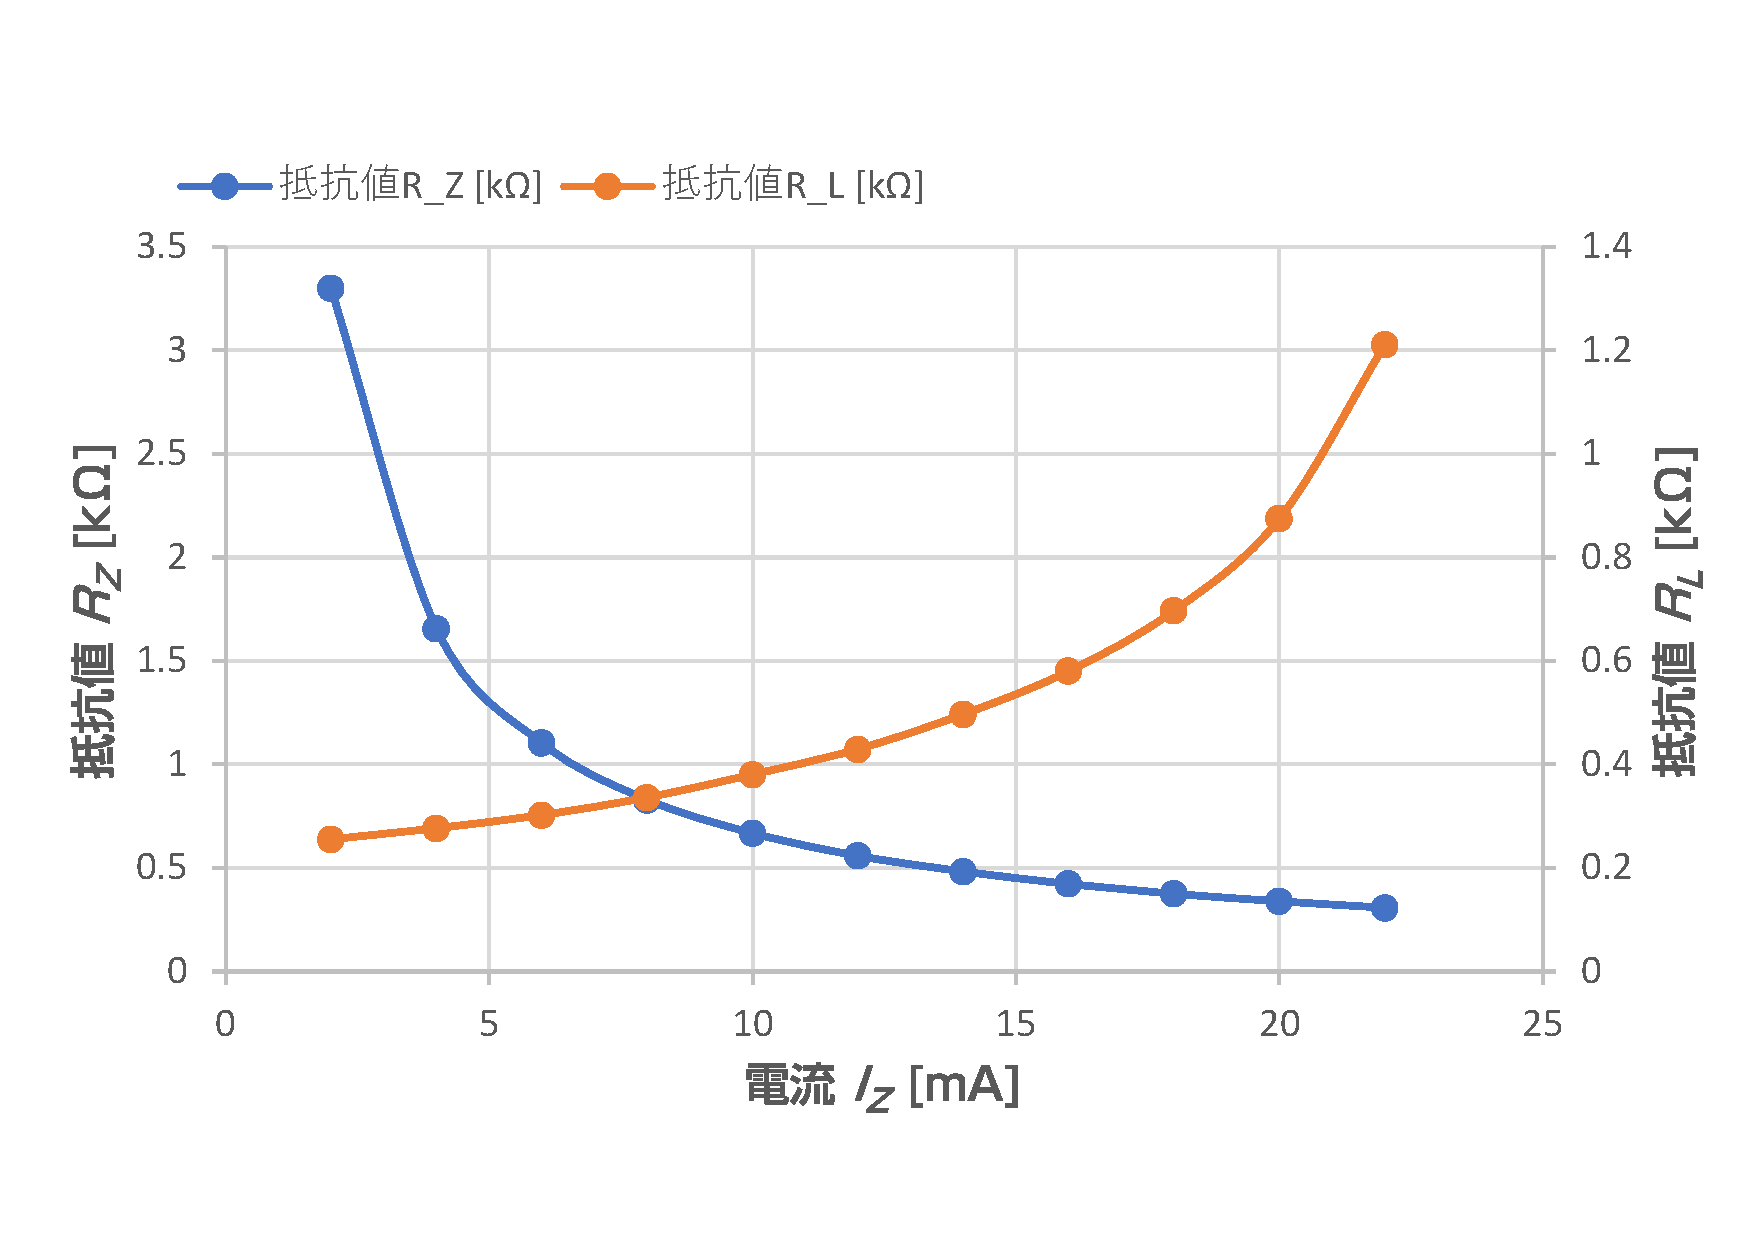
\includegraphics[width=13cm]{./figs/G-zener_IZ-RZRL.pdf}
			\caption{ツェナーダイオードの抵抗値電流特性}
			\label{fig:zener_IZ-RZRL}
		\end{figure}

	\end{enumerate}
